%\section{More non-linear recurrences}
\begin{python0}
from solutions import *; clear() 
\end{python0}

The next recurrence is different from ones you have seen earlier ...
do you see the \textit{main} difference?

\begin{eg}
Consider this:
\[
a_n = \frac{1}{n} a_{n-1} + n
\]
for $n \geq 1$ and $a_0 = 10$.
Find a closed form for $a_n$. 
\end{eg}

Quick pause ... previous recurrences look like, for instance, the following:
\[
a_n = 3 a_{n-1} + 4 a_{n-2} 
\]
which is linear and homogeneous,
or this
\[
a_n = -2 a_{n-1} + 10 a_{n-2} + n^2 + 1
\]
which is linear and nonhomogeneous,
or
\[
a_n = n a_{n-1} + 4 a_{n-2} + n^2 + 1
\]
which is nonlinear and nonhomogeneous.
In the above example, the recurrence is nonlinear and nonhomogenous, but
the multiplier in front of $a_{n-1}$ is $1/n$.
In previous nonlinear cases, the multiplier in front of $a_{n-1}$ looks like
$n$ or $(n + 1)$ or $(n^2 + 3n + 5)$, etc. -- they are polynomials in
$n$. 


Before find the closed form, of course you must do some experiments
to get some data for later testing.
Here are some test data that I'll use later:
\begin{align*}
a_0 &= 10 \\
a_1 &= 11 \\
a_2 &= \frac{1}{2} \cdot 11 + 2 = \frac{15}{2} \\
a_3 &= \frac{1}{3} \cdot \frac{15}{2} + 3 = \frac{33}{6} \\
a_4 &= \frac{1}{4} \cdot \frac{33}{6} + 4 = \frac{129}{24} \\
\end{align*}
Let
\[
f(x) = \sum_{n = 0}^\infty a_n x^n
\]
Then
\begin{align*}
f(x)
&= a_0 + \sum_{n = 1}^\infty a_n x^n \\
&= a_0 + \sum_{n = 1}^\infty \left( \frac{1}{n} a_{n-1} + n \right) x^n \\
&= a_0
  + \sum_{n = 1}^\infty \frac{1}{n} a_{n-1} x^n
  + \sum_{n = 1}^\infty  n x^n \\
&= a_0
  + \sum_{n = 1}^\infty a_{n-1} \cdot \frac{1}{n} x^{n}
  + x \sum_{n = 1}^\infty  n x^{n-1} \\
&= a_0
  + \sum_{n = 1}^\infty a_{n-1} \cdot \int_{0}^x t^{n-1} \ dt
  + x \sum_{n = 1}^\infty  \frac{d}{dx} x^n\\
&= a_0
  + \int_{0}^x \left( \sum_{n = 1}^\infty a_{n-1} t^{n-1} \right) \ dt
  + x \frac{d}{dx} \sum_{n = 1}^\infty  x^n\\
&= a_0
  + \int_0^x f(t) \ dt
  + x \frac{d}{dx} \left( \sum_{n = 0}^\infty  x^n - 1 \right) \\
&= a_0
  + \int_0^x f(t) \ dt
  + x \frac{d}{dx} \left( \frac{1}{1-x}  - 1 \right) \\
&= a_0
  + \int_0^x f(t) \ dt
  + \frac{x}{(1-x)^2}   \\
\end{align*}
Study the above very carefully.
In particular, why did I introduce the integral?
Where does the \textit{idea} come from?
If you really understood the stuff I talked about when we find closed
forms earlier, you would really know why I made the above attack on the
problem.
If you still don't see the intuition/idea:
pause and compute the closed form for this:
\[
b_n = nb_{n-1} + n
\]
for $n \geq 1$ and $b_0 = 10$ using ideas from previous sections.
OK ... move on ...

At this point we have
\[
f(x) - \int_0^x f(t) \ dt = a_0 + \frac{x}{(1-x)^2}
\]
This is an integral equation -- it contains the unknown $f(x)$
and an integral of $f(x)$.
I want to convert this to a differential equation.
Taking the derivative and replacing $f(x)$ by $y$ (to make it more
recognizable):
\[
y' - y
= \frac{d}{dx} \left( a_0 + \frac{x}{(1-x)^2} \right)
= \frac{(1-x)^2 - x \cdot 2(1-x)(-1)}{(1-x)^4} = \frac{1+x}{(1-x)^3}
\]
I get this horrific looking thingy:
\[
y' - y = \frac{1+x}{(1-x)^3}
\]
Well ... don't shout and scream ... it's actually not that bad because
this is a Bernoulli differential equation which is documented
in all standard textbooks on differential equations and you can
also find it on the web.
The solution to the above differential equation is of the form
\begin{align*}
y
&= e^x
  \left(
  \int e^{-x} \frac{1+x}{(1-x)^3} \ dx + C
  \right)
   \\
\end{align*}
where $C$ is a constant.
OK ... so we now need to compute
\[
  \int e^{-x} \frac{1+x}{(1-x)^3} \ dx
\]
The next thing to do is of course to check a table of integrals.
Unfortunately you (probably) won't find the above
in standard integral tables.

Wait ... in fact note that the original differential equation looks like this:
\[
y' - y = g'(x)
\]
where $g(x) = a_0 + x/(1-x)^2$; i.e., the right-hand-side of the differential
equation is not just any function, it's a \textit{derivative}.
Why is that important?
Because the differential equation looks like this
\[
y = e^x \left(
  \int e^{-x} g'(x) \ dx + C
  \right)
\]
and, \textit{using integration by parts},
\begin{align*}
  \int e^{-x} g'(x) \ dx
&= e^{-x} g(x) - \int g(x)(-e^{-x}) \ dx \\
&= e^{-x} g(x) + \int e^{-x} g(x) \ dx
\end{align*}
which in our case is
\begin{align*}
\int e^{-x} g'(x) \ dx
&= e^{-x} \left( a_0 + \frac{x}{(1-x)^2} \right)
+ \int e^{-x} \left( a_0 + \frac{x}{(1-x)^2} \right) \ dx
\\
&= e^{-x} \left( a_0 + \frac{x}{(1-x)^2} \right)
+ a_0(-e^{-x}) + \int e^{-x} \frac{x}{(1-x)^2}\ dx
\\
&= e^{-x} \frac{x}{(1-x)^2} 
+ \int e^{-x} \frac{x}{(1-x)^2}\ dx
\end{align*}
Now why is this a good thing?
Because we've moved from computing this:
\[
  \int e^{-x} \frac{1+x}{(1-x)^3} \ dx
\]
to computing this:
\[
\int e^{-x} \frac{x}{(1-x)^2}\ dx
\]
I don't know about you, but the second integral
definitely looks easier to me.

Now, again I don't see
\[
\int e^{-x} \frac{x}{(1-x)^2}\ dx
\]
in standard integration tables.
But I notice that the derivative of $\frac{1}{1-x}$ is $\frac{1}{(1-x)^2}$.
(Do you know why I do not try to think of \lq\lq the derivative of $-e^{-x}$ is
$e^{-x}$''?)
So I'm going to try integration by parts again:
\begin{align*}
\int e^{-x} \frac{x}{(1-x)^2}\ dx
&= \int xe^{-x} \cdot \frac{1}{(1-x)^2} \ dx \\
&= \int xe^{-x} \cdot d \left( \frac{1}{1-x} \right) \\
&= xe^{-x} \cdot \frac{1}{1-x}
   - \int \frac{1}{1-x} \cdot d \left( xe^{-x} \right)
   \\
&= xe^{-x} \cdot \frac{1}{1-x}
   - \int \frac{1}{1-x} \cdot \left( e^{-x} - xe^{-x} \right) dx
   \\
&= xe^{-x} \cdot \frac{1}{1-x}
   - \int \frac{1}{1-x} \cdot e^{-x} \left( 1 - x \right) dx
   \\
&= xe^{-x} \cdot \frac{1}{1-x}
   - \int \frac{1}{1-x} \cdot e^{-x} \left( 1 - x \right) dx
   \\
&= xe^{-x} \cdot \frac{1}{1-x}
   - \int e^{-x} dx & & \text{well ... what do you know ...}
   \\
&= xe^{-x} \cdot \frac{1}{1-x}
   + e^{-x}
   \\
&= e^{-x} \cdot \frac{x + (1-x)}{1-x}
   \\
&= e^{-x} \frac{1}{1-x}
\end{align*}


Putting the above together I get this:
\begin{align*}
\int e^{-x} g'(x) \ dx
&= e^{-x} \frac{x}{(1-x)^2} 
+ e^{-x} \frac{1}{1-x}
\\
&=  e^{-x} \frac{x + (1-x)}{(1-x)^2}
\\
&=  e^{-x} \frac{1}{(1-x)^2}
\end{align*}
Let's check:
\begin{align*}
\frac{d}{dx} \left( \frac{e^{-x}}{(x-1)^2} \right)
&= \frac{(-e^{-x}(1-x)^2 - e^{-x} \cdot 2(1-x)(-1)}{(1-x)^4} \\
&= e^{-x} \frac{-(1-x) +  2}{(1-x)^4} \\
&= e^{-x} \frac{1+x}{(1-x)^4} \\
&= e^{-x} g'(x)
\end{align*}
Looks like everything is good.
Therefore
\begin{align*}
f(x)
&= y = e^x \left( \int e^{-x} g'(x) \ dx + C \right) \\
&= e^x \left( e^{-x} \frac{1}{(1-x)^2} + C \right) \\
&= \frac{1}{(1-x)^2} + C e^x
\end{align*}

Phew!
Now ... where are we?!?

Recall that $f(x) = \sum_{n=0}^\infty a_n x^n$ and the goal is to
find a closed form for $a_n$.
First we compute $C$.
\[
10 = a_0 = f(0) = \frac{1}{(1-0)^2} + C e^{0} = 1 + C
\]
i.e., $C = 9$.
Therefore
\[
f(x)
= \frac{1}{(1-x)^2} + 9 e^{x}
\]
Since we have well--known power series for $1/(1-x)^2$ and $e^x$,
we're now in the final lap!
Onward!!!
\begin{align*}
f(x)
&= \frac{1}{(1-x)^2} + 9 e^{x} \\
&= \sum_{n=0}^\infty \binom{2 + n - 1}{n} x^n
   + 9 \sum_{n=0}^\infty \frac{1}{n!}x^n
   \\
&= \sum_{n=0}^\infty \binom{n+1}{n} x^n
   + \sum_{n=0}^\infty 9 \frac{1}{n!}x^n
   \\
&= \sum_{n=0}^\infty \binom{n+1}{1} x^n
   + \sum_{n=0}^\infty \frac{9}{n!}x^n
   \\
&= \sum_{n=0}^\infty
   \left( (n+1) 
   + \frac{9}{n!} \right)
   x^n
\end{align*}
Hence
\[
a_n = n + 1 + \frac{9}{n!}
\]
for $n \geq 0$.
Of course we have to check this closed form:
\begin{align*}
a_0 &= 0 + 1 + \frac{9}{1} = 10 \\
a_1 &= 1 + 1 + \frac{9}{1} = 11 \\
a_2 &= 2 + 1 + \frac{9}{2} = \frac{15}{2} \\
a_3 &= 3 + 1 + \frac{9}{6} = \frac{33}{6} \\
a_4 &= 4 + 1 + \frac{9}{24} = \frac{129}{24}
\end{align*}
and they all agree with the values computed using the
recursive form of $a_n$.
TADA!

I'm going to check the closed form for $n = 0, ..., 17$:
\begin{Verbatim}[frame=single, fontsize=\footnotesize]
def f(n):
    if n == 0: return 1
    else: return n * f(n - 1)

def b(n):
    return n + 1 + 9.0 / f(n)

def a(n):
    if n == 0: return 10
    else: return a(n - 1) / float(n) + n

for n in range(18):
    print('%.30f' % a(n), '%.30f' % b(n), a(n) == b(n), a(n) - b(n))
\end{Verbatim}
Here's the output:
\begin{Verbatim}[frame=single, fontsize=\footnotesize]
10.000000000000000000000000000000 10.000000000000000000000000000000 True 0.0
11.000000000000000000000000000000 11.000000000000000000000000000000 True 0.0
7.500000000000000000000000000000 7.500000000000000000000000000000 True 0.0
5.500000000000000000000000000000 5.500000000000000000000000000000 True 0.0
5.375000000000000000000000000000 5.375000000000000000000000000000 True 0.0
6.075000000000000177635683940025 6.075000000000000177635683940025 True 0.0
7.012500000000000177635683940025 7.012500000000000177635683940025 True 0.0
8.001785714285714945503968920093 8.001785714285714945503968920093 True 0.0
9.000223214285714590232601040043 9.000223214285714590232601040043 True 0.0
10.000024801587301226390991359949 10.000024801587301226390991359949 True 0.0
11.000002480158730833181834896095 11.000002480158730833181834896095 True 0.0
12.000000225468975045828301517759 12.000000225468975045828301517759 True 0.0
13.000000018789080513670342043042 13.000000018789080513670342043042 True 0.0
14.000000001445313202452780387830 14.000000001445313202452780387830 True 0.0
15.000000000103236530435424356256 15.000000000103236530435424356256 True 0.0
16.000000000006881606395836570300 16.000000000006881606395836570300 True 0.0
17.000000000000429878355134860612 17.000000000000429878355134860612 True 0.0
18.000000000000024868995751603507 18.000000000000024868995751603507 True 0.0
\end{Verbatim}

Yes!

Now I'm ready to present the solution ...

\newpage
\SOLUTION

Let
\[
f(x) = \sum_{n = 0}^\infty a_n x^n
\]
We then have
\begin{align*}
f(x)
&= a_0 + \sum_{n = 1}^\infty a_n x^n \\
&= a_0 + \sum_{n = 1}^\infty \left( \frac{1}{n} a_{n-1} + n \right) x^n \\
&= a_0
  + \sum_{n = 1}^\infty \frac{1}{n} a_{n-1} x^n
  + \sum_{n = 1}^\infty  n x^n \\
&= a_0
  + \sum_{n = 1}^\infty a_{n-1} \cdot \frac{1}{n} x^{n}
  + x \sum_{n = 1}^\infty  n x^{n-1} \\
&= a_0
  + \sum_{n = 1}^\infty a_{n-1} \cdot \int_{0}^x t^{n-1} \ dt
  + x \sum_{n = 1}^\infty  \frac{d}{dx} x^n\\
&= a_0
  + \int_{0}^x \left( \sum_{n = 1}^\infty a_{n-1} t^{n-1} \right) \ dt
  + x \frac{d}{dx} \sum_{n = 1}^\infty  x^n\\
&= a_0
  + \int_0^x f(t) \ dt
  + x \frac{d}{dx} \left( \sum_{n = 0}^\infty  x^n - 1 \right) \\
&= a_0
  + \int_0^x f(t) \ dt
  + x \frac{d}{dx} \left( \frac{1}{1-x}  - 1 \right) \\
&= a_0
  + \int_0^x f(t) \ dt
  + \frac{x}{(1-x)^2}   
\end{align*}
Therefore
\[
f(x) - \int_0^x f(t) \ dt = a_0 + \frac{x}{(1-x)^2}
\]
Taking the derivative and replacing $f(x)$ by $y$, we obtain the following
differential equation:
\[
y' - y
= g'(x)
\]
where $g(x) = a_0 + x/(1-x)^2$.
Viewing the above as a Bernoulli differential equation, 
the solution to the above differential equation is of the form
\begin{align*}
y
&= e^x
  \left(
  \int e^{-x} g'(x) \ dx + C
  \right)
   \\
   \tag{1}
\end{align*}
where $C$ is a constant.
Using integration by parts,
\begin{align*}
  \int e^{-x} g'(x) \ dx
&= e^{-x} g(x) - \int g(x)(-e^{-x}) \ dx \\
&= e^{-x} g(x) + \int e^{-x} g(x) \ dx \\
&= e^{-x} \left( a_0 + \frac{x}{(1-x)^2} \right)
   + \int e^{-x} \left( a_0 + \frac{x}{(1-x)^2} \right) \ dx
   \\
&= e^{-x} \left( a_0 + \frac{x}{(1-x)^2} \right)
   + a_0(-e^{-x}) + \int e^{-x} \frac{x}{(1-x)^2}\ dx
   \\
&= e^{-x} \frac{x}{(1-x)^2} 
   + \int e^{-x} \frac{x}{(1-x)^2}\ dx
   \tag{2}
\end{align*}
We now compute $\int e^{-x} \frac{x}{(1-x)^2}\ dx$
using integration by parts:
\begin{align*}
\int e^{-x} \frac{x}{(1-x)^2}\ dx
&= \int xe^{-x} \cdot \frac{1}{(1-x)^2} \ dx \\
&= \int xe^{-x} \cdot d \left( \frac{1}{1-x} \right) \\
&= xe^{-x} \cdot \frac{1}{1-x}
   - \int \frac{1}{1-x} \cdot d \left( xe^{-x} \right)
   \\
&= xe^{-x} \cdot \frac{1}{1-x}
   - \int \frac{1}{1-x} \cdot \left( e^{-x} - xe^{-x} \right) dx
   \\
&= xe^{-x} \cdot \frac{1}{1-x}
   - \int \frac{1}{1-x} \cdot e^{-x} \left( 1 - x \right) dx
   \\
&= xe^{-x} \cdot \frac{1}{1-x}
   - \int e^{-x} dx 
   \\
&= xe^{-x} \cdot \frac{1}{1-x}
   + e^{-x}
   \\
&= e^{-x} \cdot \frac{x + (1-x)}{1-x}
   \\
&= e^{-x} \frac{1}{1-x}
\tag{3}
\end{align*}
Substituting (3) into (2),
we obtain:
\begin{align*}
\int e^{-x} g'(x) \ dx
&= e^{-x} \frac{x}{(1-x)^2} 
+ e^{-x} \frac{1}{1-x}
\\
&=  e^{-x} \frac{x + (1-x)}{(1-x)^2}
\\
&=  e^{-x} \frac{1}{(1-x)^2}
\tag{4}
\end{align*}
Substituting (4) into (2), we have
\begin{align*}
f(x)
&= y = e^x \left( \int e^{-x} g'(x) \ dx + C \right) \\
&= e^x \left( e^{-x} \frac{1}{(1-x)^2} + C \right) \\
&= \frac{1}{(1-x)^2} + C e^x
\end{align*}
Using $a_0 = 10$, we compute $C$:
\[
10 = a_0 = f(0) = \frac{1}{(1-0)^2} + C e^{0} = 1 + C
\]
i.e., $C = 9$.
Therefore
\begin{align*}
f(x)
&= \frac{1}{(1-x)^2} + 9 e^{x} \\
&= \sum_{n=0}^\infty \binom{2 + n - 1}{n} x^n
   + 9 \sum_{n=0}^\infty \frac{1}{n!}x^n
   \\
&= \sum_{n=0}^\infty \binom{n+1}{n} x^n
   + \sum_{n=0}^\infty 9 \frac{1}{n!}x^n
   \\
&= \sum_{n=0}^\infty \binom{n+1}{1} x^n
   + \sum_{n=0}^\infty \frac{9}{n!}x^n
   \\
&= \sum_{n=0}^\infty
   \left( (n+1) 
   + \frac{9}{n!} \right)
   x^n
\end{align*}
Hence the following is a closed form for $a_n$:
\[
a_n = n + 1 + \frac{9}{n!}
\]
for $n \geq 0$.
\qed


\newpage
\begin{ex}
Note that the above recurrence looks like this:
\[
a_n = \frac{1}{n} a_{n-1} + n
\]
In particular, the multiple in front of $a_{n-1}$ is $\frac{1}{n}$
which is not constant (and therefore the recurrence is
not linear) and more importantly it's not a polynomial ...
that's the whole point of this section.
The appearance of $\frac{1}{n}$ can appear in cases where
there's an \lq\lq average'' computation.
This happens, for instance,
when $a_n$ is the average runtime of quicksort.
What do I mean by \lq\lq average'' here?
Let's look at quicksort (see section on quicksort algorithms).

Suppose the array to be sorted is \verb!x[0..(n-1)]!.
The pivot can be at \verb!x[0]! or it can be at \verb!x[1]! or ...
In any case the array is re--organized using the pivot.
Specifically,
the array is partitioned into two parts using the pivot
so that the array is re-organized into
\lq\lq left-hand-side array, pivot, right-hand-side array''.
There are several cases.
The left-hand-side array of values $\leq$ the pivot can have 0 elements.
This is followed by the pivot.
The right-hand-side array of values $>$ the pivot can have $n - 1$ values.
That's one case.
For this case, the time taken (recursively) is
\[
An + B + T(0) + T(n - 1)
\]
where $T(n)$ is the time taken to quicksort an array of size $n$.
The $An + B$ is time to scan the array
and place the values of the array into the structure
of 
\lq\lq left-hand side array, pivot, right-hand side array''.
Another case is when the left-hand-side array has 1 value.
This is followed by the pivot and then followed by the right-hand-side
array which has $n - 2$ values.
In this case, the time taken (recursively) is
\[
An + B + T(1) + T(n - 2)
\]
The time taken when the left-hand-side array has 2 values is
\[
An + B + T(2) + T(n - 3)
\]
Etc.
When we take the average over all $n$ cases, we get
\begin{align*}
T(n)
&= An + B \\
&\textwhite{= \ }
+ \frac{1}{n} 
\biggl(
  \left( T(0) + T(n-1) \right)
  + \left( T(1) + T(n-2) \right)
  + \cdots
  + \left( T(n - 1) + T(0) \right)
\biggr) \\
&= An + B + \frac{1}{n}\sum_{i=0}^{n-1} \left( T(i) + T(n - 1 - i) \right)
\end{align*}
Of course $T(0) = T(1) = C$ where $C$ is a constant.
Note that, if you're sharp, you realized that I'm assuming that the
values in the array \verb!x! are unique.
Furthermore, I'm assuming all the above cases are equally likely.

In the above, you can see that each $T(i)$ appears twice.
So I can simplify it a little like this:
\begin{align*}
T(n)
&= An + B + \frac{2}{n}\sum_{i=0}^{n-1} T(i)
\end{align*}
\end{ex}

As you can see this recursion involves $\frac{1}{n}$ as coefficient
In fact the above is more complicated than the first example of this section.
Why? Because
\begin{align*}
T(n)
&= An + B + \frac{2}{n}\sum_{i=0}^{n-1} T(i)
\end{align*}
does not have a (fixed) degree.
\qed

\newpage
\begin{ex}
  In the above, I computed
  \[
  \int e^{-x} g'(x) \ dx 
  \]
  using (basically) two integration by parts.
  Is it possible to simplify the above
  by doing one integration by parts?
  \qed
\end{ex}


\newpage
\begin{ex}
  One of the above computation involves an integral of the form
  \[
  \int e^{-x} \frac{\text{?}}{(1-x)^2} \ dx
  \]
  How far can you go in generalizing the earlier computation?
  Find all possible ? so that the above integral
  can be computed.
  What about
  \[
  \int e^{-x} \frac{\text{?}}{(?-x)^2} \ dx
  \]
  Or this
  \[
  \int e^{?x} \frac{\text{?}}{(?-x)^2} \ dx
  \]
  Or this
  \[
  \int e^{?x} \frac{\text{?}}{(?-?x)^2} \ dx
  \]
  Or how about this:
  \[
  \int e^{?x} \frac{\text{?}}{(?-?x)^?} \ dx
  \]
  State the most general version of your theorem ... and prove it.
  \qed
\end{ex}


\newpage
\begin{ex}
  The differential equation
  \[
  y' - y = g'(x) = \frac{1+x}{(1-x)^3}
  \]
  is a degree one linear nonhomogeneous differential equation.
  Can you compute the solution viewing the differential equation this way?
  (In other words don't view the equation as a Bernoulli differential
  equation.)
  \qed
\end{ex}





\begin{comment}
Can we find the closed form using an ad-hoc method?
\begin{align*}
a_n
&= \frac{1}{n} a_{n-1} + n \\
&= \frac{1}{n} \left( \frac{1}{n-1} a_{n-2} + n - 1 \right) + n \\
&= \frac{1}{n(n-1)} a_{n-2} + \frac{n - 1}{n} + n \\
&= \frac{1}{n(n-1)}
   \left(
     \frac{1}{n-2} a_{n-3} + n - 2
   \right)
   + \frac{n - 1}{n} + n \\
&= \frac{1}{n(n-1)(n-2)} a_{n-3}
   + \frac{n - 2}{n(n-1)} 
   + \frac{n - 1}{n} + n \\
&= \frac{1}{n(n-1)(n-2)}
   \left(
     \frac{1}{n-3} a_{n-4} + n - 3 
   \right)
   + \frac{n - 2}{n(n-1)} 
   + \frac{n - 1}{n} + n \\
&= \frac{1}{n(n-1)(n-2)(n-3)} a_{n-4}
   + \frac{n - 3}{n(n-1)(n-2)} 
   + \frac{n - 2}{n(n-1)} 
   + \frac{n - 1}{n} + n \\
&= \ldots \\
&= \frac{1}{n(n-1)(n-2)(n-3)\cdots(1)} a_{0}
\\
   &\hspace{1cm} + \frac{n - 3}{n(n-1)(n-2)} 
   + \frac{n - 2}{n(n-1)} 
   + \frac{n - 1}{n} + n \\
\end{align*}
\end{comment}


\newpage
\begin{ex}
  Study this:
  \[
  a_n = \frac{c}{n} a_{n - 1} + dn
  \]
  where $a_0 = e$.
  Here $c,d,e$ are constants.
  \qed
\end{ex}

\newpage
\begin{ex}
  What about this:
  \[
  a_n = \frac{1}{n + 1} a_{n - 1} + n^2 + 1
  \]
  where $a_0 = 1$?
  \qed
\end{ex}



\newpage
\begin{ex}
  Or this:
  \[
  a_n = \frac{1}{n - 1} a_{n - 1} + n^2 + n
  \]
  where $a_0 = 1$?
  \qed
\end{ex}

\newpage
\begin{ex}
  Or this:
  \[
  a_n = \frac{1}{n^2} a_{n - 1} + 3
  \]
  where $a_0 = 2$?
  \qed
\end{ex}



\newpage
\begin{ex}
  Now try this:
  \[
  a_n = \frac{1}{n^2 - 1} a_{n - 1} + 5n
  \]
  where $a_0 = 3$?
  \qed
\end{ex}

\newpage
\begin{ex}
  And this:
  \[
  a_n = \frac{1}{n^2 + 1} a_{n - 1} + 5n^2
  \]
  where $a_0 = 7$?
  \qed
\end{ex}


\newpage
\begin{ex}
Analyze this problem:
Find a closed form for $a_n$ where
\[
a_n = \frac{p(n)}{q(n)} a_{n - 1} + r(n)
\]
where $p(n), q(n), r(n)$ are polynomials (in $n$).
The method used in the first problem of this section relies
heavily on your ability (luck?) of integrating complex looking functions.
The smart (and deep) question is to ask what functions can be integrated?
What functions cannot be integrated? In fact what do you mean by
\lq\lq can be integrated''?
Do some research on this and write a paper.
\qed
\end{ex}


\newpage
\begin{ex}
What about something like this:
\[
a_n = \frac{2}{n} \sum_{i=0}^{n-1} a_i 
\]
\qed
\end{ex}


\newpage
\begin{ex}
Can you handle this:
\[
a_n = An + B + \frac{2}{n} \sum_{i=0}^{n-1} a_i 
\]
where $a_0$ is given?
\qed
\end{ex}
  

\newpage
Let
\[
a_n = An + B + \frac{2}{n} \sum_{i=0}^{n-1} a_i
\]
for $n \geq 1$ 
and $a_0 = C$.

Numerically, for testing purposes let $A = B = C = 1$.
Then
\begin{align*}
a_0 &= 1 \\
a_1 &= 1 + 1 + \frac{2}{1} \left( 1 \right) = 4 \\
a_2 &= 2 + 1 + \frac{2}{2} \left( 1 + 4\right) = 8 
\end{align*}
Algebraically, we have the following cases:
\begin{align*}
  a_1
  &= A + B + \frac{2}{1} (a_0) \\
  &= A + B + 2a_0 \\
  a_2 &= 2A + B + \frac{2}{2}(a_0 + a_1)  \\
      &= 2A + B + (a_0 + A + B + 2 a_0) \\
      &= 3A + 2B + 3 a_0
\end{align*}

Recall that 
\[
\frac{1}{1-x} \sum_{n=0}^\infty c_n x^n
= \sum_{n=0}^\infty \left( \sum_{i=0}^n c_i \right) x^n
\]
Note that for $n > 0$
\[
a_n
= An + B + \frac{2}{n} \sum_{i=0}^{n-1} a_i
= \sum_{i=0}^{n-1} \left( A + \frac{B}{n} + \frac{2a_i}{n} \right)
\]
Let
\[
f(x) = \sum_{n=0}^\infty a_n x^n
\]
Then
\begin{align*}
f(x)
&= a_0 + \sum_{n=1}^\infty a_n x^n
= a_0 +
   \sum_{n=1}^\infty
   \left(
     \sum_{i=0}^{n-1} \left( A + \frac{B}{n} + \frac{2a_i}{n} \right)
   \right) x^n
   \\
&= a_0 +
   x
   \sum_{n=1}^\infty
   \left(
     \sum_{i=0}^{n-1} \left( A + \frac{B}{n} + \frac{2a_i}{n} \right)
   \right) x^{n - 1}
   \\
&= a_0 +
   x
   \sum_{m=0}^\infty
   \left(
     \sum_{i=0}^{m} \left( A + \frac{B}{m+1} + \frac{2a_i}{m+1} \right)
   \right) x^{m}
   \\
&= a_0 +
   x
   \frac{1}{1 - x}
   \sum_{m=0}^\infty
     \left( A + \frac{B}{m+1} + \frac{2a_m}{m+1} \right)
     x^{m}
   \\
&= a_0 +
   \frac{x}{1 - x}
   \left(
   \sum_{m=0}^\infty A x^m
   + \sum_{m=0}^\infty \frac{B}{m + 1} x^m
   + \sum_{m=0}^\infty \frac{2a_m}{m+1} x^m
     \right)
   \\
&= a_0
   + \frac{x}{1 - x}
   \left(
   A \sum_{n=0}^\infty x^n
   + \frac{1}{x} \sum_{m=0}^\infty \frac{B}{m + 1} x^{m+1}
   + \frac{1}{x} \sum_{m=0}^\infty \frac{2a_m}{m+1} x^{m+1}
   \right)
   \\
&= a_0
   + \frac{x}{1 - x}
   \left(
   A \frac{1}{1-x}
   + \frac{1}{x} \sum_{m=0}^\infty B \int_{t=0}^x t^m \ dt
   + \frac{1}{x} \sum_{m=0}^\infty 2a_m \int_{t=0}^x t^m \ dt
   \right)
   \\
&= a_0
   + \frac{x}{1 - x}
   \left(
   \frac{A}{1-x}
   + \frac{B}{x} \int_{t=0}^x \sum_{m=0}^\infty  t^m \ dt
   + \frac{2}{x} \int_{t=0}^x \sum_{m=0}^\infty a_m  t^m \ dt
   \right)
   \\
&= a_0
   + \frac{x}{1 - x}
   \left(
   \frac{A}{1-x}
   + \frac{B}{x} \int_{t=0}^x \frac{1}{1-t} \ dt
   + \frac{2}{x} \int_{t=0}^x f(t) \ dt
   \right)
   \\
&= a_0
   + A \frac{x}{(1-x)^2}
   + \frac{B}{1-x} \int_{t=0}^x \frac{1}{1-t} \ dt
   + \frac{2}{1-x} \int_{t=0}^x f(t) \ dt
   \\
\end{align*}
Therefore
\[
(1 - x)f(x) - 2 \int_{t=0}^x f(t) \ dt
= a_0(1-x)
  + A \frac{x}{1-x}
  + B \int_{t=0}^x \frac{1}{1-t} \ dt
\]
Taking derivative, we get
\begin{align*}
-f(x) + (1-x)f'(x) - 2f(x)
&= -a_0
  + A \frac{1(1-x) - x(-1)}{(1-x)^2}
  + B \frac{1}{1-x}
\\
\THEREFORE
(1 - x)f'(x) - 3f(x) 
&= -a_0
  + A \frac{1}{(1-x)^2}
  + B \frac{1}{1-x}
\\
&= \frac{-a_0(1-x)^2 + A + B(1-x)}{(1-x)^2}
\\
&= \frac{-a_0x^2 + (2 a_0 - B) x + (-a_0 + A + B)}{(1-x)^2}
\\
f'(x) - \frac{3}{1-x}f(x) 
&= \frac{-a_0x^2 + (2 a_0 - B) x + (-a_0 + A + B)}{(1-x)^3}
\end{align*}
Hence $f(x)$ is the solution to
the following Bernoulli differential equation:
\[
y' - \frac{3}{1-x} y 
= \frac{-a_0x^2 + (2 a_0 - B) x + (-a_0 + A + B)}{(1-x)^3}
\]
Therefore
\begin{align*}
f(x) &= \frac
       {
         \displaystyle\int m(x)
         \left(
           \frac{-a_0x^2 + (2 a_0 - B) x + (-a_0 + A + B)}{(1-x)^3}
           \right) \ dx
           + C
       }
       {  m(x) }
\end{align*}
where
$C$ is a constant.
and
\[
m(x)
= e^{ \int \left( -\frac{3}{1-x} \right) \ dx}
= e^{ 3 \ln (1 - x) }
= (1 - x)^3
\]
So
\begin{align*}
f(x)
&= \frac
{
  \displaystyle\int (1-x)^3
  \left(
    \frac{-a_0x^2 + (2 a_0 - B) x + (-a_0 + A + B)}{(1-x)^3}
  \right) \ dx + C
}
{ (1-x)^3 } 
\\
&= \frac
{
  \displaystyle\int 
  \left(
    -a_0x^2 + (2 a_0 - B) x + (-a_0 + A + B)
  \right) \ dx + C
}
{ (1-x)^3 }
\\
&=
\frac{1}{(1-x)^3}
\left(
    -\frac{a_0}{3}x^3 + \frac{2 a_0 - B}{2}x^2 + (-a_0 + A + B )x + C
\right)
\end{align*}
To solve for $C$, we use $f(0) = a_0$:
\[
a_0 = f(0) = \frac{1}{(1-0)^3} \left( 0 + 0 + 0 + C \right)
\]
i.e., $C = a_0$.

Now we expand the right-hand-side into power series:
\begin{align*}
&f(x) =
\left(
    -\frac{a_0}{3}x^3 + \frac{2 a_0 - B}{2}x^2 + (-a_0 + A + B )x + a_0
\right)
\sum_{n=0}^\infty \binom{3 + n - 1}{n} x^n
\\
&=
\left(
    -\frac{a_0}{3}x^3 + \frac{2 a_0 - B}{2}x^2 + (-a_0 + A + B )x + a_0
\right)
\sum_{n=0}^\infty \binom{n + 2}{n} x^n
\\
&=
\left(
    -\frac{a_0}{3}x^3 + \frac{2 a_0 - B}{2}x^2 + (-a_0 + A + B )x + a_0
\right)
\sum_{n=0}^\infty \binom{n + 2}{2} x^n
\\
&=
  -\frac{a_0}{3} \sum_{n=0}^\infty \binom{n + 2}{2} x^{n+3} 
 + \frac{2 a_0 - B}{2} \sum_{n=0}^\infty \binom{n + 2}{2} x^{n+2} \\
&\hspace{1cm} + (-a_0 + A + B ) \sum_{n=0}^\infty \binom{n + 2}{2} x^{n+1}
+ a_0 \sum_{n=0}^\infty \binom{n + 2}{2} x^{n} 
\\
&=
  -\frac{a_0}{3} \sum_{n=3}^\infty \binom{n - 1}{2} x^{n} 
  + \frac{2 a_0 - B}{2} \sum_{n=2}^\infty \binom{n}{2} x^{n} \\
&\hspace{1cm} + (-a_0 + A + B ) \sum_{n=1}^\infty \binom{n + 1}{2} x^{n}
+ a_0 \sum_{n=0}^\infty \binom{n + 2}{2} x^{n} 
\\
&= a_0 \binom{2}{2}
+ \left( a_0 \binom{3}{2} + (-a_0 + A + B) \binom{2}{2}\right) x
\\
&\hspace{1cm} + \left( a_0 \binom{4}{2} + (-a_0 + A + B) \binom{3}{2} +
  \frac{2a_0 - B}{2}\binom{2}{2}
  \right) x^2
  \\
&\hspace{1cm} + \sum_{n=3}^\infty
   \left(
     -\frac{a_0}{3}\binom{n-1}{2}
     + \frac{2a_0 - B}{2} \binom{n}{2}
     + (-a_0 + A + B)\binom{n+1}{2}
     + a_0 \binom{n+2}{2}
   \right) x^n
\\
&= a_0
+ \left( 3 a_0 + (-a_0 + A + B) \right) x
\\
&\hspace{1cm} + \left( 6 a_0 + 3(-a_0 + A + B)  +
  \frac{2a_0 - B}{2}
  \right) x^2
  \\
&\hspace{1cm} + \sum_{n=3}^\infty
   \left(
     -\frac{a_0}{3}\binom{n-1}{2}
     + \frac{2a_0 - B}{2} \binom{n}{2}
     + (-a_0 + A + B)\binom{n+1}{2}
     + a_0 \binom{n+2}{2}
   \right) x^n
\\
&= a_0
+ \left( A + B + 2a_0 \right) x
\\
&\hspace{1cm} + \left( 3A + \frac{5}{2}B + 4a_0 \right) x^2 \\
&\hspace{1cm} + \sum_{n=3}^\infty
   \left(
     -\frac{a_0}{3}\binom{n-1}{2}
     + \frac{2a_0 - B}{2} \binom{n}{2}
     + (-a_0 + A + B)\binom{n+1}{2}
     + a_0 \binom{n+2}{2}
   \right) x^n
\end{align*}

At this point, notice that the closed form derived is incorrect.
Your job is to find the error.


\SOLUTION.

The above is incorrect because of the following step:
\begin{align*}
  f(x) &= ... \\
&= a_0 +
   x
   \sum_{m=0}^\infty
   \left(
     \sum_{i=0}^{m} \left( A + \frac{B}{m+1} + \frac{2a_i}{m+1} \right)
   \right) x^{m}
   \\
&= a_0 +
   x
   \frac{1}{1 - x}
   \sum_{m=0}^\infty
     \left( A + \frac{B}{m+1} + \frac{2a_m}{m+1} \right)
     x^{m}
   \\
&= ...
\end{align*}
Basically 
\[
c_{i,m} = A + \frac{B}{m+1} + \frac{2a_i}{m+1}
\]
is a term of two variables.
The following is correct
\[
\frac{1}{1-x}
\sum_{n=0}^\infty c_{n,n} x^n
=
\sum_{n=0}^\infty
\left(
  \sum_{i = 0}^n c_{i,i}
\right) x^n
\]
But the following is wrong
\[
\frac{1}{1 - x}
\sum_{n=0}^\infty c_{n,n} x^n
=
\sum_{n=0}^\infty
  \left(
  \sum_{i=0}^n c_{i,n}
  \right) x^n
\]
This incorrect version is used in the computations above.


\newpage
Let's analyze the following recurrence carefully:
\[
a_n = An + B + \frac{2}{n} \sum_{i=0}^{n-1} a_i
\]
I will assume that there's only one base condition: $a_0$ is given.
For instance $a_1$ is computed using the above recurrence like this:
\[
a_1 = A + B + \frac{2}{1} a_0 = A + B + 2 a_0
\]
(For the case of quicksort, there are usually \textit{two} base conditions, i.e., $a_0$
and $a_1$ are given -- this will be an exercise later.)
Multiplying the above recurrence by $n$, I get 
\[
na_n = An^2 + Bn + 2 \sum_{i=0}^{n-1} a_i \tag{1}
\]
Here's the crucial step:
We also have
\[
(n-1)a_{n-1} = A(n-1)^2 + B(n-1) + 2 \sum_{i=0}^{n-2} a_i \tag{2}
\]
Using that, (1) $-$ (2) gives us
\begin{align*}
na_n - (n-1)a_{n-1}
&= A(n^2 - (n-1)^2) + B(n - (n-1)) + 2a_{n-1} \\
&= (2n - 1) A + B + 2a_{n-1}
\end{align*}
Why is this step a reasonable strategy?
Because the sum $\sum_{i=0}^{n-1} a_i$ has too many $a_i$'s -- I want to get rid of them as fast
as possible.
And you also now understand why I had to multiple the first recurrence by
$n$. (What will happen if I don't?)

(ASIDE:
In case you're thinking I'm just pulling algebraic tricks like that
out of thin air, then think again: it's not entirely new.
The above trick is analogous to the method used in
one of the standard derivations of the geometric sum formula.
Here's the derivation.
Let $S = 1 + r + r^2 + \cdots + r^n$. Notice that there's a summation.
Then $rS = r + r^2 + r^3 + \cdots r^{n+1}$.
This is also a summation.
But notice that many of the terms in the two summations are the same.
On subtraction, we get
\[
rS - S = r^{n+1} - 1
\]
Notice that the summation disappears - get it now?
After that it's easy: we get
\[
(r-1)S = r^{n+1} - 1
\]
and therefore
\[
S = \frac{r^{n+1} - 1}{r - 1}
\]
i.e.,
\[
1 + r + r^2 + \cdots + r^n = \frac{r^{n+1} - 1}{r - 1}
\]
See the magic now?
This is a very important trick in removing summations ... and it's not new.)

And now finally I get this:
\begin{align*}
na_n 
&= (2n - 1) A + B + 2a_{n-1} + (n-1)a_{n-1} \\
&= (2n - 1) A + B + (n+1)a_{n-1} \\
\THEREFORE
a_n
&= \left(2 - \frac{1}{n}\right) A + \frac{1}{n}B +
   \left( 1 + \frac{1}{n} \right) a_{n-1}
   \\
&= 2A + \frac{1}{n}(B - A) +
   \left( 1 + \frac{1}{n} \right) a_{n-1}
\end{align*}
To make life easier, I'm going to let $C = B - A$ and $D = 2A$.
Then I get
\[
a_n
= C\frac{1}{n} + D
   + \left( 1 + \frac{1}{n} \right) a_{n-1}
\]
Note that this is a recurrence of degree 1.
The original recurrence
\[
a_n = An + B + \frac{2}{n} \sum_{i=0}^{n-1} a_i
\]
has degree $n$.

Let
\[
f(x) = \sum_{n = 0}^\infty a_n
\]
Then
\begin{align*}
f(x)
&= a_0 + \sum_{n = 1}^\infty a_n x^n \\
&= a_0 + \sum_{n = 1}^\infty
   \left( C\frac{1}{n} + D
   + \left( 1 + \frac{1}{n} \right) a_{n-1}\right) x^n
 \\
&= a_0
   + C \sum_{n=1}^\infty \frac{1}{n} x^n
   + D \sum_{n=1}^\infty  x^n
   + \sum_{n=1}^\infty a_{n-1} x^n
   + \sum_{n=1}^\infty a_{n-1} \frac{1}{n} x^n
   \\
&= a_0
   + C \sum_{n=1}^\infty \int_{t=0}^x t^{n-1} \ dt
   + D \left( \frac{1}{1-x} - 1 \right)
   + x \sum_{n=1}^\infty a_{n-1} x^{n-1}
   + \sum_{n=1}^\infty a_{n-1} \int_{t=0}^x t^{n-1} \ dt
   \\
&= a_0
   + C \int_{t=0}^x  \left( \sum_{n=1}^\infty t^{n-1} \right) \ dt
   + D \frac{x}{1-x}
   + x \sum_{n=0}^\infty a_n x^n
   +   \int_{t=0}^x \left(\sum_{n=1}^\infty  a_{n-1} t^{n-1}\right) \ dt
   \\
&= a_0
   + C \int_{t=0}^x  \left( \sum_{n=0}^\infty t^{n} \right) \ dt
   + \frac{Dx}{1-x}
   + x f(x)
   +   \int_{t=0}^x \left(\sum_{n=0}^\infty  a_{n} t^{n}\right) \ dt
   \\
&= a_0
   + C \int_{t=0}^x  \frac{1}{1-t} \ dt
   + \frac{Dx}{1-x}
   + x f(x)
   +  \int_{t=0}^x f(t) \ dt
\end{align*}
Therefore we get this
\[
(1-x)f(x) - \int_{t=0}^x f(t) \ dt
= a_0
   + C \int_{t=0}^x  \frac{1}{1-t} \ dt
   + \frac{Dx}{1-x}
\]
Taking derivatives on both sides:
\begin{align*}
  -f(x) + (1-x)f'(x) - f(x)
  &= \frac{C}{1-x} + D\frac{(1-x) - x(-1)}{(1-x)^2}\\
\THEREFORE (1 - x) f'(x) - 2 f(x) &= \frac{C}{1-x} + D\frac{1}{(1-x)^2}\\
\THEREFORE f'(x) - \frac{2}{1-x} f(x)
&= \frac{C}{(1-x)^2} 
+ \frac{D}{(1-x)^3}
\end{align*}
Therefore viewing $f(x)$ as a solution to the following Bernoulli differential equation,
\[
y' - \frac{2}{1-x} y  = \frac{C}{(1-x)^2}  + \frac{D}{(1-x)^3}
\]
we get
\[
f(x) = \frac{\int m(x) q(x) \ dx + E}{m(x)}
\]
where $E$ is a constant,
\[
m(x) = e^{\int \frac{-2}{1 - x} \ dx}
\]
and $q(x) = \frac{C}{(1-x)^2} + D\frac{1}{(1-x)^3}$.
We have
\[
m(x)
= e^{\int \frac{-2}{1 - x} \ dx}
= e^{2 \int \frac{1}{1 - x} d(1-x)}
= e^{2 \ln (1 - x)}
= (1-x)^2
\]
Therefore
\begin{align*}
f(x)
&= \frac{1}{(1-x)^2}
   \left(
     \int (1-x)^2
     \left(
       \frac{C}{(1-x)^2} + \frac{D}{(1-x)^3}
     \right) \ dx + E 
   \right)
   \\
&= \frac{1}{(1-x)^2}
   \left(
     \int \left( C + \frac{D}{1-x} \right) \ dx + E
   \right)
   \\
&= \frac{1}{(1-x)^2}
   \left(
     C x 
     - D \ln (1-x)
     + E
   \right)
   \\
&=     \frac{Cx}{(1-x)^2} 
     - D \frac{\ln (1-x)}{(1-x)^2}
     + \frac{E}{(1-x)^2}
     \\
&=     \frac{Cx + E}{(1-x)^2} 
     - D \frac{\ln (1-x)}{(1-x)^2}
\end{align*}
The constant $E$ can be computed easily: Substituting $x = 0$, we get
\[
a_0 = f(0) = 0 +  E - 0
\]
i.e.,
\[
E = a_0
\]

The following is a well--known power series for $\ln (1 - x)$:
\[
\ln (1-x) = - \sum_{n=1}^\infty \frac{1}{n} x^n
\]
Therefore
\begin{align*}
-\frac{\ln (1-x)}{(1-x)^2}
&= \left( -\ln (1-x) \right) \cdot \frac{1}{(1-x)^2} \\
&= - \left( -\sum_{n=1}^\infty \frac{1}{n} x^n \right) \cdot
   \sum_{n=0}^\infty (n+1) x^n
   \\
&= \sum_{n=1}^\infty \frac{1}{n} x^n  \cdot
   \sum_{n=0}^\infty (n+1) x^n
\end{align*}
I'll show you that the big-$\Theta$ of the coefficients of the power
series of this function is $n \ln n$; all the other functions
have power series with \lq\lq smaller'' coefficients.
In fact I'll do better than that: I'll derive an exact closed form for
coefficients of the power series for $-\ln(1-x)/(1-x)^2$ and then for $f(x)$.

The $n$--th coefficient of the above power series
\[
\sum_{n=1}^\infty \frac{1}{n} x^n  \cdot
\sum_{n=0}^\infty (n+1) x^n
\]
is
\[
b_n =
0 \cdot (n+1) + \frac{1}{1} \cdot n + \frac{1}{2} \cdot (n-1) +
\cdots + \frac{1}{n} \cdot (1)
= \frac{n}{1} + \frac{n-1}{2} + \cdots + \frac{1}{n}
\]
Finding an exact  closed form for this is difficult ... to say the least.
Also, note that in the section on products of power series,
as much as possible we in fact do \textit{not} want to compute the above expression
doing term-by-term multiplication.
For instance if you have the following product of power series:
\[
\sum_{n=1}^\infty x^n
\sum_{n=0}^\infty (n+1)x^n
\]
you should not multiply out term-by-term.
You should do this instead:
\begin{align*}
\sum_{n=1}^\infty x^n
\sum_{n=0}^\infty (n+1)x^n
&=
x\sum_{n=0}^\infty x^n
\sum_{n=0}^\infty (n+1)x^n
\\
&= x \frac{1}{1-x}\frac{1}{(1-x)^2} \\
&= x \frac{1}{(1-x)^3} \\
&= x \sum_{n=0}^\infty \binom{n+2}{2} x^n \\
&= ...
\end{align*}
Right?

However in the expression above
\[
-\frac{\ln (1-x)}{(1-x)^2}
\]
there's no easy way to write $\ln (1-x)$ into something that will multiply
easily with $\frac{1}{(1-x)^2}$ or vice versa.
So we are forced to compute the coefficient of $x^n$ \lq\lq by hand'', term-by-term.
It's not really as hopeless as you think.
Watch this:
\begin{align*}
b_n
&= \frac{n}{1} + \frac{n-1}{2} + \cdots + \frac{1}{n}
\\
&= \frac{n - 0}{1} + \frac{n - 1}{2} + \frac{n - 2}{3} + \cdots +
   \frac{n - (n-1)}{n} \\
&= \left(
   \frac{n}{1} + \frac{n}{2} + \frac{n}{3} + \ldots + \frac{n}{n}
   \right)
   -
   \left( \frac{1}{2} + \frac{2}{3} + \frac{3}{4} + \cdots + \frac{n-1}{n}
   \right)
   \\   
&= \left(
   {1} + \frac{1}{2} + \frac{1}{3} + \ldots + \frac{1}{n}
   \right) n
   -
   \left( \frac{1}{2} + \frac{2}{3} + \frac{3}{4} + \cdots + \frac{n-1}{n}
   \right)
\end{align*}
The sequence
\[
H_n = 1 + \frac{1}{2} + \frac{1}{3} + \ldots + \frac{1}{n}
\]
is well--known -- this sum is called the harmonic sum.
In particular
\[
H_n - \ln n \rightarrow \gamma
\]
as $n \rightarrow \infty$
where $\gamma$ is a constant of value $0.577...$;
$\gamma$ is called the Euler's constant for harmonic sums.
Even more precisely, it's known that
\[
H_n = \ln n + \gamma + \ep_n
\]
where $\ep_n$ is approximately $1/(2n) - 1/(12n^2)$.
(See below.)
As for
\[
\frac{1}{2} + \frac{2}{3} + \frac{3}{4} + \cdots + \frac{n-1}{n}
\]
again, the harmonic sum is actually lurking around:
\begin{align*}
\frac{1}{2} + \frac{2}{3} + \frac{3}{4} + \cdots + \frac{n-1}{n}
&= \frac{2-1}{2} + \frac{3-1}{3} + \frac{4-1}{4} + \cdots + \frac{n - 1)}{n}\\
&=
\left( 1 - \frac{1}{2} \right)
+ \left( 1 - \frac{1}{3} \right)
+ \left( 1 - \frac{1}{4} \right)
+ \cdots
+ \left( 1 - \frac{1}{n} \right)
\\
&= (n - 1) - (H_n - 1) \\
&= n - H_n
\end{align*}
Therefore altogether here's what I can tell you about $b_n$:
\begin{align*}
  b_n =
&= n H_n - (n - H_n) \\
&= (n + 1) H_n - n \\
&= (n + 1) (\ln n + \gamma + \ep_n) - n \\
&= n \ln n + (\gamma - 1) n + \ln n + n \ep_n + \gamma + \ep_n
\end{align*}
which has a big-$\Theta$ of $n\ln n$.

Let's get on with the power series of $f(x)$.
\begin{align*}
f(x)
&= \frac{Cx + E}{(1-x)^2}
  + D \sum_{n=1}^\infty b_n x^n
  \\
&=
  (Cx + E)\sum_{n=0}^\infty (n + 1)x^n
  + D \sum_{n=1}^\infty b_n x^n
  \\
&=
  \sum_{n=0}^\infty C(n + 1)x^{n+1}
  + \sum_{n=0}^\infty E(n + 1)x^n
  + \sum_{n=1}^\infty Db_n x^n
  \\
&=
  \sum_{n=1}^\infty Cn x^n
  + E + \sum_{n=1}^\infty E(n + 1)x^n
  + \sum_{n=1}^\infty Db_n x^n
  \\
&= E + \sum_{n=1}^\infty \left( Cn + E(n+1) + D b_n \right) x^n
\end{align*}
The $n$--th coefficient for $n > 0$ is
\begin{align*}
&Cn + E(n+1) + Db_n
\\
&= (C + E)n
   + E
   + D
   \left(
     n \ln n + (\gamma - 1) n + \ln n + n \ep_n + \gamma + \ep_n
   \right)
   \\   
&= D n \ln n + (C + E + D(\gamma - 1)) n + D\ln n + \left(E + D(n \ep_n + \gamma)\right) + D\ep_n
\end{align*}
Let's not forget that $C = B - A$, $D = 2A$, and $E = a_0$:
\begin{align*}
An + &B + \frac{2}{n} \sum_{i=0}^{n-1} a_i \\
&= 2A n \ln n \\
&\hspace{1cm} + (B - A + a_0 + 2A(\gamma - 1)) n \\
&\hspace{1cm} + 2A\ln n \\
&\hspace{1cm} + \left(a_0 + 2A(n \ep_n + \gamma)\right) \\
&\hspace{1cm} + 2A\ep_n
\end{align*}
Note that this is \textit{not} an approximation or some
big-O/big-$\Theta$ thingy -- it's exact.
Even if we repllace $\ep_n$ with $1/(2n)$,
the right-hand side is still a very good approximation to the right.
In particular, note that 
\[
An + B + \frac{2}{n} \sum_{i=0}^{n-1} a_i = \Theta(n \ln n)
\]
In fact we even know the constant of the big-$\Theta$.
Therefore I can be even more precise:
\[
An + B + \frac{2}{n} \sum_{i=0}^{n-1} a_i =
2A n \ln n + \Theta(n)
\]

Here's a test:
\begin{Verbatim}[frame=single, fontsize=\footnotesize]
import math

e = math.e
def ln(x):
    x = float(x)
    return math.log(x, e)

a0 = 1.0
A =  1.0
B = -1.0
gamma = 0.5772156649

table_a = {0:a0}
def a(n):
    if not table_a.has_key(n):
        s = 0.0
        for i in range(n):
            s += a(i)
        table_a[n] = A * n + B + (2.0 / n) * s
    return table_a[n]

def ep(n):
    return 1.0/(2.0*n) - 1.0/(12.0*n*n) + 1.0/(120.0*n**4)

def b(n):
    if n == 0: return a0
    t0 = 2 * A * n * ln(n)
    t1 = (B - A + a0 + 2 * A * (gamma - 1)) * n
    t2 = 2 * A * ln(n)
    t3 = (a0 + 2 * A * (n * ep(n) + gamma))
    t4 = 2 * A * ep(n)
    return t0 + t1 + t2 + t3 + t4

for n in range(1, 100):
    print('%5s' % n, '%10.5f' % a(n), '%10.5f' % b(n), '%15.12f' % (a(n)-b(n)))
\end{Verbatim}
Here's the output
\begin{Verbatim}[frame=single, fontsize=\footnotesize, commandchars=\\\{\}]
    1    2.00000    2.00886 -0.008862659600
    2    4.00000    4.00030 -0.000302072760
    3    6.66667    6.66671 -0.000039266405
    4    9.83333    9.83334 -0.000009114366
    5   13.40000   13.40000 -0.000002928009
    6   17.30000   17.30000 -0.000001157628
    7   21.48571   21.48571 -0.000000528491
    8   25.92143   25.92143 -0.000000268102
    9   30.57937   30.57937 -0.000000147415
   10   35.43730   35.43730 -0.000000086367
 \textit{snipped}   
   30  158.68920  158.68920 -0.000000000242
   31  165.74369  165.74369 -0.000000000188
   32  172.86068  172.86068 -0.000000000143
   33  180.03828  180.03828 -0.000000000105
   34  187.27470  187.27470 -0.000000000072
   35  194.56826  194.56826 -0.000000000045
   36  201.91738  201.91738 -0.000000000021
   37  209.32055  209.32055 -0.000000000001
   38  216.77636  216.77636  0.000000000017
   39  224.28344  224.28344  0.000000000032
   40  231.84053  231.84053  0.000000000046
   41  239.44640  239.44640  0.000000000059
   42  247.09988  247.09988  0.000000000070
 \textit{snipped}
   86  619.50162  619.50162  0.000000000265
   87  628.59934  628.59934  0.000000000268
   88  637.71979  637.71979  0.000000000271
   89  646.86271  646.86271  0.000000000275
   90  656.02785  656.02785  0.000000000278
   91  665.21497  665.21497  0.000000000281
   92  674.42383  674.42383  0.000000000284
   93  683.65419  683.65419  0.000000000287
   94  692.90583  692.90583  0.000000000290
   95  702.17852  702.17852  0.000000000293
   96  711.47205  711.47205  0.000000000296
   97  720.78620  720.78620  0.000000000299
   98  730.12075  730.12075  0.000000000302
   99  739.47550  739.47550  0.000000000306
\end{Verbatim}

OK ... let's tidy up what we have ...

\newpage

First I'm going to assume the following without proof:

\begin{thm}
Let $H_n$ be the $n$--th harmonic sum, i.e.,
\[
H_n = 1 + \frac{1}{2} + \cdots \frac{1}{n}
\]
$\gamma$ be Euler's
constant for harmonic series, i.e.,
\[
\gamma = \lim_{n \rightarrow \infty} \left( \sum_{i=1}^n \frac{1}{k} - \ln n \right)
= 0.577...
\]
and $\ep_n$ be the $n$--th error term
of the harmonic series according to the following:
\[
H_n - \ln n = \gamma + \ep_n
\]
Then, asymptotically,
\[
\ep_n \sim \frac{1}{2n} - \frac{1}{12n^2} + \frac{1}{120 n^4} - \frac{1}{252 n^6} - \cdots
\]
\qed
\end{thm}

(The infinite sum on the right can actually be specified explicitly, but I'm not
going to. 
Don't get me wrong: it's an interesting series.
However I won't be using it in this set of notes.
To find out more, refer to my notes on analytic number theory.)

When I write
\[
f(n) \sim g(n)
\]
and say that $f(n)$ and $g(n)$ are \defterm{asymptotically equivalent},
I mean \lq\lq $f(n)$ and $g(n)$ are more or less the same when $n \rightarrow \infty$''.
The intuition is that when $n$ gets larger and larger, $f(n)$ and $g(n)$ get closer
and closer to each other.
To be precise (mathematically speaking), $f(n) \sim g(n)$ means
\[
\lim_{n \rightarrow \infty} \frac{f(n)}{g(n)} = 1
\]
Like other asymptotics (big-O, big-$\Theta$, etc.) asymptotic equivalence
was originally used by people studying number theory, especially analytic number theory.
Concretely speaking, here's how to think about asymptotic equivalence.
You know that
\[
n^2 = O(n^3)
\]
In fact
\[
5n^2 = O(1.5n^3)
\]
The tightest power you can get for the upper bound is 2:
\[
5n^2 = O(1.5n^2)
\]
As for big--$\Theta$ we have
\[
5n^2 = \Theta(10.5 n^1)
\]
The tightest you can get for the lower bound is 2:
\[
5n^2 = \Theta(10.5 n^2)
\]
Combining the two,
\[
5n^2 = \Theta(n^2)
\]
However $\Theta$ ignores constants so that the following are true:
\[
5 n^2 + 10n + 1= \Theta(2.3 n^2 + 0.1 n + 3.5)
\]
and
\[
2.3 n^2 + 10n + 1 = \Theta(2.3 n^2 + 0.1 n + 3.5)
\]
Asymptotic equivalence is stronger in the sense that
\[
2.3 n^2 + 10n + 1 \sim 2.3 n^2 + 0.1 n + 3.5
\]
So asymptotic equivalence focuses on the \lq\lq most significant term'' of the sum
\textit{and} its coefficient as well.
The above is an over--simplification but will be helpful in seeing the big picture.

OK .... let's get back to the main theorem:

\begin{thm}
  Let
  \[
  a_n = An + B + \frac{2}{n} \sum_{i=0}^{n-1} a_i
  \]
  for $n > 0$.
  Then 
  \begin{align*}
  a_n = 2A n \ln n &+ (B - A + a_0 + 2A(\gamma - 1)) n \\
    &+ 2A\ln n 
 + \left(a_0 + 2A(n \ep_n + \gamma)\right) 
 + 2A\ep_n
 \end{align*}
 In particular
   \[
  a_n = 2A n \ln n + \Theta(n)
  \]

\end{thm}

\proof


\newpage
\begin{ex}
What happens if there are \textit{two} base considiions, i.e.,
$a_0$ and $a_1$ are given and
\[
a_n = An + B + \frac{2}{n} \sum_{i=0}^{n-1} a_i
\]
for $n \geq 2$?
\qed
\end{ex}

\newpage
\begin{ex}
  Let's see if you can find the closed form or big-$\Theta$ or big-O of this:
  \[
  a_n = An + B + n \sum_{i=0}^{n-1} a_i
  \]
  for $n \geq 1$ where $a_0$ is given.
\qed
\end{ex}

\newpage
\begin{ex}
  Can you handle this:
  \[
  a_n = An^2 + Bn + C + \frac{2}{n} \sum_{i=0}^{n-1} a_i, \,\,\,\,\, n > 0
  \]
  where $a_0$ is given.
  \qed
\end{ex}


\newpage
\begin{ex}
  Can you handle this:
  \[
  a_n = An + B + \frac{2}{n} \sum_{i=0}^{n-1} (i + 1) a_i
  \]
  where $n > 0$. Assume that $a_0$ is given.
  \qed
\end{ex}

\newpage
\begin{ex}
  Suppose you have a recurrence of the form
  \[
  a_n = f(n) + g(n) \sum_{i=0}^{n-1} h(i) a(i)
  \]
  for $n > n_0$ 
  where $f(n), g(n), h(n)$ are functions with $g(n) \neq 0$ for all $n > n_0$.
  Convert the recurrence to another of degree 1.
  \qed
\end{ex}

\SOLUTION

Let $n > n_0$.
Dividing the given recurrence by $g(n)$, we get
\[
  \frac{1}{g(n)} a_n = \frac{f(n)}{g(n)} + \sum_{i=0}^{n-1} h(i) a(i) \tag{1}
\]
We also have
\[
  \frac{1}{g(n-1)} a_{n-1} = \frac{f(n-1)}{g(n-1)} + \sum_{i=0}^{n-2} h(i) a(i) \tag{2}
\]
(1) $-$ (2) give us
\begin{align*}
  \frac{1}{g(n)} a_n - \frac{1}{g(n-1)} a_{n-1}
  &= \frac{f(n)}{g(n)} - \frac{f(n-1)}{g(n-1)} + h(n-1) a_{n-1} \\
  \THEREFORE
  \frac{1}{g(n)} a_n 
  &= \frac{f(n)}{g(n)} - \frac{f(n-1)}{g(n-1)} + h(n-1) a_{n-1} + \frac{1}{g(n-1)} a_{n-1}\\
  &= \frac{f(n)}{g(n)} - \frac{f(n-1)}{g(n-1)} + \left( h(n-1) + \frac{1}{g(n-1)} \right)
  a_{n-1}
  \\
  \THEREFORE
  a_n 
  &= f(n) - \frac{f(n-1)g(n)}{g(n-1)} + g(n)\left( h(n-1) + \frac{1}{g(n-1)} \right)
  a_{n-1}\\
\end{align*}
which is clearly a degree 1 recurrence.
\qed

\newpage
\begin{ex}
  Design a quicksort that partitions not into twwo parts but into three.
  Program it (and test it of course).
  Compute the average runtime.
  \qed
\end{ex}

\newpage
\subsection*{Solutions}

\newpage
\section*{Solutions}
Solution to Exercise \ref{ex:dfa0}\labeltext{}{sol:dfa0}.

\tinysidebar{\debug{exercises/{dfa0/answer.tex}}}

    Solution not provided.
    

\newpage

Solution to Exercise \ref{ex:dfa1}\labeltext{}{sol:dfa1}.

\tinysidebar{\debug{exercises/{dfa1/answer.tex}}}
  The ID computation is
  \begin{align*}
    (q_0, aba)
    &\vdash (\delta(q_0, a), ba) = (q_0, ba) \\ 
    &\vdash (\delta(q_0, b), a) = (q_1, a) \\
    &\vdash (\delta(q_1, a), \ep) = (q_0, \ep)
  \end{align*}
  $q_0$ is not an accept state. Therefore $aba$ is not accepted.


\newpage

Solution to Exercise \ref{ex:dfa4}\labeltext{}{sol:dfa4}.

\tinysidebar{\debug{exercises/{dfa4/answer.tex}}}

    Solution not provided.
    

\newpage

Solution to Exercise \ref{ex:dfa5}\labeltext{}{sol:dfa5}.

\tinysidebar{\debug{exercises/{dfa5/answer.tex}}}

    Solution not provided.
    

\newpage

Solution to Exercise \ref{ex:implementing-a-single-dfa0}\labeltext{}{sol:implementing-a-single-dfa0}.

\tinysidebar{\debug{exercises/{implementing-a-single-dfa0/answer.tex}}}

    Solution not provided.
    

\newpage

Solution to Exercise \ref{ex:nfastatediag0}\labeltext{}{sol:nfastatediag0}.

\tinysidebar{\debug{exercises/{nfastatediag0/answer.tex}}}

    Solution not provided.
    

\newpage

Solution to Exercise \ref{ex:nfastatediag1}\labeltext{}{sol:nfastatediag1}.

\tinysidebar{\debug{exercises/{nfastatediag1/answer.tex}}}

    Solution not provided.
    

\newpage

Solution to Exercise \ref{ex:nfastatediag2}\labeltext{}{sol:nfastatediag2}.

\tinysidebar{\debug{exercises/{nfastatediag2/answer.tex}}}

    Solution not provided.
    

\newpage

Solution to Exercise \ref{ex:nfastatediag3}\labeltext{}{sol:nfastatediag3}.

\tinysidebar{\debug{exercises/{nfastatediag3/answer.tex}}}

    Solution not provided.
    

\newpage

Solution to Exercise \ref{ex:nfastatediag4}\labeltext{}{sol:nfastatediag4}.

\tinysidebar{\debug{exercises/{nfastatediag4/answer.tex}}}

    Solution not provided.
    

\newpage

Solution to Exercise \ref{ex:nfastatediag5}\labeltext{}{sol:nfastatediag5}.

\tinysidebar{\debug{exercises/{nfastatediag5/answer.tex}}}

    Solution not provided.
    

\newpage

Solution to Exercise \ref{ex:nfastatediag6}\labeltext{}{sol:nfastatediag6}.

\tinysidebar{\debug{exercises/{nfastatediag6/answer.tex}}}

    Solution not provided.
    

\newpage

Solution to Exercise \ref{ex:nfastatediag7}\labeltext{}{sol:nfastatediag7}.

\tinysidebar{\debug{exercises/{nfastatediag7/answer.tex}}}

    Solution not provided.
    

\newpage

Solution to Exercise \ref{ex:nfastatediag8}\labeltext{}{sol:nfastatediag8}.

\tinysidebar{\debug{exercises/{nfastatediag8/answer.tex}}}

    Solution not provided.
    

\newpage

Solution to Exercise \ref{ex:nfastatediag9}\labeltext{}{sol:nfastatediag9}.

\tinysidebar{\debug{exercises/{nfastatediag9/answer.tex}}}

    Solution not provided.
    

\newpage

Solution to Exercise \ref{ex:nfastatediag10}\labeltext{}{sol:nfastatediag10}.

\tinysidebar{\debug{exercises/{nfastatediag10/answer.tex}}}

    Solution not provided.
    

\newpage

Solution to Exercise \ref{ex:nfastatediag11}\labeltext{}{sol:nfastatediag11}.

\tinysidebar{\debug{exercises/{nfastatediag11/answer.tex}}}

    Solution not provided.
    

\newpage

Solution to Exercise \ref{ex:nfastatediag12}\labeltext{}{sol:nfastatediag12}.

\tinysidebar{\debug{exercises/{nfastatediag12/answer.tex}}}

    Solution not provided.
    

\newpage

Solution to Exercise \ref{ex:nfastatediag13}\labeltext{}{sol:nfastatediag13}.

\tinysidebar{\debug{exercises/{nfastatediag13/answer.tex}}}

    Solution not provided.
    

\newpage

Solution to Exercise \ref{ex:nfa0}\labeltext{}{sol:nfa0}.

\tinysidebar{\debug{exercises/{nfa0/answer.tex}}}
The formal definition of this NFA is $(\Sigma, Q, q_0, \delta, F)$ where
\begin{tightlist}
\li $\Sigma = \{a,b\}$
\li $Q = \{q_0\}$
\li $\delta$ is the function
\[
\delta : Q \times \Sigma_\epsilon \rightarrow P(Q)
\]
given by
\begin{align*}
  \delta(q_0, \epsilon) &= \{\} \\
  \delta(q_0, a) &= \{\} \\
  \delta(q_0, b) &= \{\} 
\end{align*}
\end{tightlist}


\newpage

Solution to Exercise \ref{ex:nfa1}\labeltext{}{sol:nfa1}.

\tinysidebar{\debug{exercises/{nfa1/answer.tex}}}

    Solution not provided.
    

\newpage

Solution to Exercise \ref{ex:nfa2}\labeltext{}{sol:nfa2}.

\tinysidebar{\debug{exercises/{nfa2/answer.tex}}}

    Solution not provided.
    

\newpage

Solution to Exercise \ref{ex:nfa3}\labeltext{}{sol:nfa3}.

\tinysidebar{\debug{exercises/{nfa3/answer.tex}}}

    Solution not provided.
    

\newpage

Solution to Exercise \ref{ex:nfa4}\labeltext{}{sol:nfa4}.

\tinysidebar{\debug{exercises/{nfa4/answer.tex}}}

    Solution not provided.
    

\newpage

Solution to Exercise \ref{ex:nfa5}\labeltext{}{sol:nfa5}.

\tinysidebar{\debug{exercises/{nfa5/answer.tex}}}

    Solution not provided.
    

\newpage

Solution to Exercise \ref{ex:dfa-as-powerful-as-nfa0}\labeltext{}{sol:dfa-as-powerful-as-nfa0}.

\tinysidebar{\debug{exercises/{dfa-as-powerful-as-nfa0/answer.tex}}}
Here's the solution.
Let $\delta$ denote the transition function of $N$.
Note that 
\begin{align*}
  \delta(q_0, \epsilon) = \{\} \\
  \delta(q_0, a) = \{\} \\
  \delta(q_0, b) = \{\} 
\end{align*}
First of all the states are labeled as all the subsets of $\{q_0\}$.


\begin{center}
\begin{tikzpicture}[>=triangle 60,shorten >=0.5pt,node distance=2cm,auto,initial text=, double distance=2pt]
\node[state] (A) at (  0,  0) {$\{q_0\}$};
\node[state] (B) at (  3,  0) {$\{\}$};

\path[->]

;
\end{tikzpicture}
\end{center}
    


The start state is the $\epsilon$-closure of $\{q_0\}$.
However in $N$, there are no $\epsilon$--transitions out of 
$q_0$.
So the $\epsilon$-closure of $\{q_0\}$ is in fact $\{q_0\}$, i.e.
$\overline{\{q_0\}} = \{q_0\}$
The $\DFA$ is now this:


\begin{longtable}{|r||r|r|r|r|r|}
\hline 
         & $w_1$ & $w_2$ & $w_3$ & $w_4$ & $\ldots$ \\ \hline \hline 
$M_1$    &       &       &       &       &          \\ \hline 
$M_2$    &       &       &       &       &          \\ \hline 
$M_3$    &       &       &       &       &          \\ \hline 
$M_4$    &       &       &       &       &          \\ \hline 
$\ldots$ &       &       &       &       &          \\ \hline 
\end{longtable}
        


Now I will compute the $a$--transition of the state $\{q_0\}$.
Let $\delta^\DFA$ denote the transition function of the $\DFA$
that we're building.
Then
\begin{align*}
\delta( \{q_0, a\} ) 
&= \overline{ \bigcup_{q \in \{q_0\}} \delta(q, a)} \\
&= \overline{ \delta(q_0, a) } \\
&= \overline{ \emptyset } \\
&= \emptyset
\end{align*}
The (incomplete) $\DFA$ now looks like this:


\begin{longtable}{|r||r|r|r|r|r|}
\hline 
         & $w_1$ & $w_2$ & $w_3$ & $w_4$ & $\ldots$ \\ \hline \hline 
$M_1$    & 0     & 0     & 1     & 0     & ...      \\ \hline 
$M_2$    & 1     & 0     & 1     & 1     & ...      \\ \hline 
$M_3$    & 0     & 1     & 1     & 1     & ...      \\ \hline 
$M_4$    & 1     & 0     & 1     & 1     & ...      \\ \hline 
$\ldots$ &       &       &       &       &          \\ \hline 
\end{longtable}
        


Using the same reasoning we have

\begin{center}
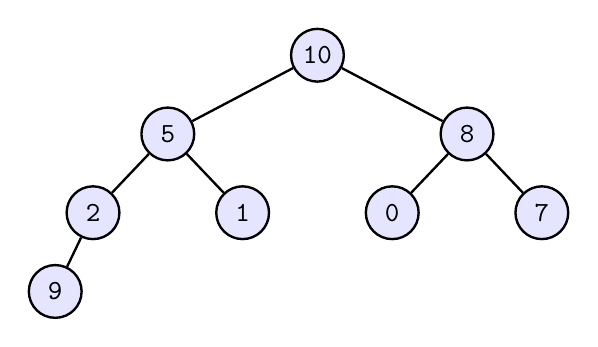
\begin{tikzpicture}

\fill[blue!10] (0.0, 0.0) circle (0.35);
\node [line width=0.03cm,black,minimum size=0.6699999999999999cm,draw,circle] at (0.0,0.0)(10){};\draw (0.0, 0.0) node[color=black] {\texttt{10}};
\fill[blue!10] (-1.9, -1.0) circle (0.35);
\node [line width=0.03cm,black,minimum size=0.6699999999999999cm,draw,circle] at (-1.9,-1.0)(5){};\draw (-1.9, -1.0) node[color=black] {\texttt{5}};
\fill[blue!10] (1.9, -1.0) circle (0.35);
\node [line width=0.03cm,black,minimum size=0.6699999999999999cm,draw,circle] at (1.9,-1.0)(8){};\draw (1.9, -1.0) node[color=black] {\texttt{8}};
\fill[blue!10] (-2.85, -2.0) circle (0.35);
\node [line width=0.03cm,black,minimum size=0.6699999999999999cm,draw,circle] at (-2.85,-2.0)(2){};\draw (-2.85, -2.0) node[color=black] {\texttt{2}};
\fill[blue!10] (-0.95, -2.0) circle (0.35);
\node [line width=0.03cm,black,minimum size=0.6699999999999999cm,draw,circle] at (-0.95,-2.0)(1){};\draw (-0.95, -2.0) node[color=black] {\texttt{1}};
\fill[blue!10] (0.95, -2.0) circle (0.35);
\node [line width=0.03cm,black,minimum size=0.6699999999999999cm,draw,circle] at (0.95,-2.0)(0){};\draw (0.95, -2.0) node[color=black] {\texttt{0}};
\fill[blue!10] (2.85, -2.0) circle (0.35);
\node [line width=0.03cm,black,minimum size=0.6699999999999999cm,draw,circle] at (2.85,-2.0)(7){};\draw (2.85, -2.0) node[color=black] {\texttt{7}};
\fill[blue!10] (-3.33, -3.0) circle (0.35);
\node [line width=0.03cm,black,minimum size=0.6699999999999999cm,draw,circle] at (-3.33,-3.0)(9){};\draw (-3.33, -3.0) node[color=black] {\texttt{9}};\draw[line width=0.03cm,black] (10) to  (5);
\draw[line width=0.03cm,black] (10) to  (8);
\draw[line width=0.03cm,black] (5) to  (2);
\draw[line width=0.03cm,black] (5) to  (1);
\draw[line width=0.03cm,black] (8) to  (0);
\draw[line width=0.03cm,black] (8) to  (7);
\draw[line width=0.03cm,black] (2) to  (9);
\end{tikzpicture}

\end{center}



It's easy to see that in the DFA, the $a$--
and $b$--transitions from the state $\{\}$ goes back to itself.
Therefore the completed DFA is this:


\begin{center}
\begin{tikzpicture}[>=triangle 60,shorten >=0.5pt,node distance=2cm,auto,initial text=, double distance=2pt]
\node[state,initial] (A) at (  0,  0) {$\{q_0\}$};
\node[state] (B) at (  3,  0) {$\{\}$};

\path[->]
(A) edge [bend left=0,pos=0.5,above] node {$a,b$} (B)
(B) edge [loop above] node {$a,b$} ()

;
\end{tikzpicture}
\end{center}
    



\newpage

Solution to Exercise \ref{ex:dfa-as-powerful-as-nfa1}\labeltext{}{sol:dfa-as-powerful-as-nfa1}.

\tinysidebar{\debug{exercises/{dfa-as-powerful-as-nfa1/answer.tex}}}

    Solution not provided.
    

\newpage

Solution to Exercise \ref{ex:dfa-as-powerful-as-nfa2}\labeltext{}{sol:dfa-as-powerful-as-nfa2}.

\tinysidebar{\debug{exercises/{dfa-as-powerful-as-nfa2/answer.tex}}}

    Solution not provided.
    

\newpage

Solution to Exercise \ref{ex:dfa-as-powerful-as-nfa3}\labeltext{}{sol:dfa-as-powerful-as-nfa3}.

\tinysidebar{\debug{exercises/{dfa-as-powerful-as-nfa3/answer.tex}}}

    Solution not provided.
    

\newpage

Solution to Exercise \ref{ex:dfa-as-powerful-as-nfa4}\labeltext{}{sol:dfa-as-powerful-as-nfa4}.

\tinysidebar{\debug{exercises/{dfa-as-powerful-as-nfa4/answer.tex}}}

    Solution not provided.
    

\newpage

Solution to Exercise \ref{ex:closure0}\labeltext{}{sol:closure0}.

\tinysidebar{\debug{exercises/{closure0/answer.tex}}}

    Solution not provided.
    

\newpage

Solution to Exercise \ref{ex:closure1}\labeltext{}{sol:closure1}.

\tinysidebar{\debug{exercises/{closure1/answer.tex}}}

    Solution not provided.
    

\newpage

Solution to Exercise \ref{ex:closure2}\labeltext{}{sol:closure2}.

\tinysidebar{\debug{exercises/{closure2/answer.tex}}}

    Solution not provided.
    

\newpage

Solution to Exercise \ref{ex:closure3}\labeltext{}{sol:closure3}.

\tinysidebar{\debug{exercises/{closure3/answer.tex}}}

    Solution not provided.
    

\newpage

Solution to Exercise \ref{ex:closure4}\labeltext{}{sol:closure4}.

\tinysidebar{\debug{exercises/{closure4/answer.tex}}}

    Solution not provided.
    

\newpage

Solution to Exercise \ref{ex:closure5}\labeltext{}{sol:closure5}.

\tinysidebar{\debug{exercises/{closure5/answer.tex}}}

    Solution not provided.
    

\newpage

Solution to Exercise \ref{ex:closure6}\labeltext{}{sol:closure6}.

\tinysidebar{\debug{exercises/{closure6/answer.tex}}}

    Solution not provided.
    

\newpage

Solution to Exercise \ref{ex:closure7}\labeltext{}{sol:closure7}.

\tinysidebar{\debug{exercises/{closure7/answer.tex}}}

    Solution not provided.
    

\newpage

Solution to Exercise \ref{ex:closure8}\labeltext{}{sol:closure8}.

\tinysidebar{\debug{exercises/{closure8/answer.tex}}}

    Solution not provided.
    

\newpage

Solution to Exercise \ref{ex:closure9}\labeltext{}{sol:closure9}.

\tinysidebar{\debug{exercises/{closure9/answer.tex}}}

    Solution not provided.
    

\newpage

Solution to Exercise \ref{ex:closure10}\labeltext{}{sol:closure10}.

\tinysidebar{\debug{exercises/{closure10/answer.tex}}}

    Solution not provided.
    

\newpage

Solution to Exercise \ref{ex:closure11}\labeltext{}{sol:closure11}.

\tinysidebar{\debug{exercises/{closure11/answer.tex}}}

    Solution not provided.
    

\newpage

Solution to Exercise \ref{ex:closure12}\labeltext{}{sol:closure12}.

\tinysidebar{\debug{exercises/{closure12/answer.tex}}}

    Solution not provided.
    
 % input solutions.tex
